\documentclass[25pt, a0paper, portrait, margin=0mm, innermargin=15mm, blockverticalspace=15mm, colspace=15mm]{tikzposter}

\usepackage[utf8]{inputenc}
\usepackage{amsmath, amssymb}
\usepackage{graphicx}
\usepackage{booktabs}
\usepackage{enumitem}
\setlist{leftmargin=1.2em, itemsep=0.3em}

% ---------- Theme ----------
\usetheme{Simple}
\usecolorstyle{Denmark}
\usebackgroundstyle{Default}
\usetitlestyle{Filled}
\useblockstyle{Default}

% ---------- Title ----------
\title{\parbox{0.85\linewidth}{\centering STLRocket: Explainable Time Series Classification via STL Quantitative Semantics}}
\author{Alessandro Della Siega\textsuperscript{1}, Second Author\textsuperscript{2}, Third Author\textsuperscript{1}}
\institute{\textsuperscript{1}University / Lab Name \quad \textsuperscript{2}Other Institution \quad \texttt{email@institution.edu}}
\titlegraphic{%
  % \includegraphics[height=6cm]{logo1.png}\hspace{20cm}\includegraphics[height=6cm]{logo2.png}
}

% Placeholder box for figures (replace with \includegraphics)
\newcommand{\figph}[2][0.9\linewidth]{%
  \begin{center}\fbox{\parbox[c][#2][c]{#1}{\centering\Large Figure placeholder}}\end{center}}

\begin{document}
\maketitle


\begin{columns}

% ===== Column 1 =====
\column{0.5}

\block{Motivation}{
  \begin{itemize}
    \item Multivariate time series classifiers are accurate but opaque.
    \item \textbf{ROCKET} \cite{rocket} is the strongest such family: thousands of
          \emph{random convolutional kernels} feed a linear classifier, giving
          state-of-the-art accuracy at very low training cost. But a learned
          kernel is an uninterpretable weight vector --- it says \emph{that} a
          pattern matters, never \emph{what} it means.
    \item Post-hoc attribution (saliency, Anchors \cite{anchors}) highlights
          \emph{where} the model looked, but produces no statement a domain
          expert can read, check, or falsify.
    \item Explanations should be \textbf{human-readable temporal properties}.
    \item \textbf{Signal Temporal Logic (STL)} \cite{stl} expresses such
          properties; its quantitative semantics (\textbf{robustness} $\rho$)
          measures how much a signal satisfies them.
  \end{itemize}
}

\block{Contributions}{
  \begin{itemize}
    \item \textbf{STL features:} random STL formulae replace ROCKET's random kernels.
    \item \textbf{Sparse interpretable classifier:} LASSO multinomial logistic regression selects few relevant concepts.
    \item \textbf{Explanations:} local and global explanations as STL formulae, built directly from the weights.
    \item \textbf{Cost of interpretability quantified:} $-2.1$ accuracy points
          against ROCKET on average, while every selected feature is a readable
          temporal property.
  \end{itemize}
}

\block{Method}{
  \textbf{1. Formula generation.} Sample $M$ formulae recursively (max depth $d_{\max}$) from
  \[
    \varphi ::= x_v \le \theta \mid x_v > \theta \mid \neg\varphi \mid \varphi\wedge\varphi \mid \varphi\vee\varphi \mid G_{[a,b]}\varphi \mid F_{[a,b]}\varphi \mid \varphi\, U_{[a,b]}\, \varphi
  \]
  \textbf{2. Features extraction.} Robustness at $t=0$, then standardized:
  \[
    x_i = \big(\rho(\tau_i,\varphi_1),\dots,\rho(\tau_i,\varphi_M)\big)^\top
  \]
  \textbf{3. LASSO multinomial logistic regression.} No intercept, trained with \texttt{glmnet} \cite{glmnet}:
  \[
    \min_{W}\; -\frac{1}{N}\sum_{i}\sum_{k} y_{i,k}\log P(y_i{=}k\mid \hat{x}_i) + \lambda\sum_{k,j}|w_{k,j}|
  \]
  $\lambda$ is chosen by cross-validation on balanced accuracy. The resulting
  $W$ is \emph{extremely} sparse: on BasicMotions only $4$ of $4\times10^4$
  entries are non-zero, so each class is decided by a handful of formulae.

\textbf{4. Building Explanations.}

  \textbf{Score} of formula $j$ for predicted class $k$:
  \[
    s_j = (w_{k,j} - \bar{w}_j)\,\hat{x}_j
  \]
  \textbf{Reparametrization:} shift thresholds so $\rho=0$ lies midway between medians of class $k$ and its nearest competitor.\\[0.5em]
  \textbf{Local explanation:} greedy conjunction of top-scoring reparametrized formulae ($\tilde{\varphi}$):
  \[
    \rho(L(\tau),\tau)>0, \quad \mathrm{Precision}(L(\tau))>\alpha, \quad L(\tau) = \bigwedge_{\varphi\in \mathrm{Selected}}\tilde{\varphi}
  \]
  \textbf{Global explanation:} $G(k) = \bigvee_{i:\, g(\hat{x}_i)=k} L(\tau_i)$,
  then simplified by removing disjuncts that agree on the training set.
}


% ===== Column 2 =====
\column{0.5}

\block{Experimental Setup}{
  \begin{itemize}
    \item \textbf{Data:} 10 multivariate UEA archive datasets \cite{uea}, using
          the archive train/test split. Wide coverage: $12$--$204$ training series,
          $3$--$1345$ channels, length $30$--$2500$, $2$--$12$ classes.
    \item \textbf{Baselines:} \textsc{ROCKET}+ridge \cite{rocket} (black-box
          reference) and \textsc{STL}+decision tree (interpretable model on the
          same STL features, isolating the classifier head).
    \item \textbf{Metrics:} balanced accuracy (classifier), precision (local), F1 (global).
    \item \textbf{Protocol:} $10$ seeds per configuration; mean $\pm$ std reported.
          Explanations are built once per dataset at its best configuration.
    \item \textbf{Ablations:} $M\in\{10,10^2,10^3,10^4\}$, Until weight
          $w_U\in\{0,1\}$, $d_{\max}\in\{1,2,3\}$.
    \item \textbf{Selected configuration:} $M=10^4$, $w_U=0$, $d_{\max}$ chosen
          per dataset. Until never helped, so it is disabled throughout.
  \end{itemize}
}

\block{Results}{

\begin{center}
\begin{tabular}{lccc}
\toprule
Dataset & STLDecisionTree & ROCKET & STLRocket \\
\midrule
BasicMotions & 92.5 $\pm$ 4.4 & \textbf{97.5 $\pm$ 0.0} & 97.0 $\pm$ 2.0 \\
Cricket & 83.8 $\pm$ 4.4 & \textbf{99.2 $\pm$ 0.7} & 94.3 $\pm$ 2.0 \\
DuckDuckGeese & 46.4 $\pm$ 5.0 & 49.6 $\pm$ 4.1 & \textbf{52.6 $\pm$ 10.6} \\
ERing & 76.2 $\pm$ 6.0 & \textbf{95.9 $\pm$ 0.5} & 86.5 $\pm$ 6.1 \\
Epilepsy & 85.4 $\pm$ 3.5 & \textbf{97.1 $\pm$ 0.6} & 96.3 $\pm$ 1.4 \\
HandMovementDirection & 30.8 $\pm$ 5.2 & 41.7 $\pm$ 3.3 & \textbf{51.3 $\pm$ 6.2} \\
Heartbeat & 60.9 $\pm$ 2.0 & 55.2 $\pm$ 1.5 & \textbf{65.4 $\pm$ 2.0} \\
RacketSports & 72.8 $\pm$ 4.7 & \textbf{89.6 $\pm$ 1.3} & 84.6 $\pm$ 2.1 \\
StandWalkJump & 36.0 $\pm$ 11.0 & \textbf{53.3 $\pm$ 3.1} & 36.0 $\pm$ 5.6 \\
UWaveGestureLibrary & 67.9 $\pm$ 3.3 & \textbf{91.9 $\pm$ 0.4} & 85.6 $\pm$ 1.3 \\
\midrule
Mean & 65.3 & \textbf{77.1} & 75.0 \\
\bottomrule
\end{tabular}

\vspace{1cm}
{Mean percentual balanced accuracy $\pm$ standard deviation; best per dataset in bold.
As expected, we lose some accuracy with respect to the ROCKET black-box classifier
($-2.1$ points on average), but STLRocket wins on $3/10$ datasets and clearly
outperforms the interpretable STL+tree baseline ($+9.7$ points).}
\end{center}

\vspace{1cm}

\begin{center}
\begin{tabular}{lcccc}
\toprule
& \multicolumn{2}{c}{Local explanations} & \multicolumn{2}{c}{Global explanations} \\
\cmidrule(lr){2-3} \cmidrule(lr){4-5}
Dataset & Mean Precision & Mean Depth & Mean F1 score & Mean Depth \\
\midrule
BasicMotions & 89.8 & 2.3 & 82.9 & 1.8 \\
Cricket & 88.7 & 2.8 & 75.9 & 2.5 \\
DuckDuckGeese & 81.7 & 2.0 & 38.2 & 2.6 \\
ERing & 97.2 & 2.3 & 70.4 & 1.5 \\
Epilepsy & 91.3 & 2.2 & 85.3 & 4.0 \\
HandMovementDirection & 84.1 & 4.2 & 39.2 & 12.0 \\
Heartbeat & 80.0 & 5.0 & 60.0 & 7.0 \\
RacketSports & 86.7 & 2.7 & 69.6 & 4.8 \\
StandWalkJump & 66.7 & 2.0 & 41.9 & 2.0 \\
UWaveGestureLibrary & 92.2 & 3.1 & 70.3 & 4.0 \\
\midrule
Mean & 85.8 & 2.9 & 63.4 & 4.2 \\
\bottomrule
\end{tabular}

\vspace{1cm}
{Explanation quality at the selected configuration. Local explanations are
\textbf{precise and small} --- $85.8\%$ precision at depth $2.9$, i.e. a formula a
reader can check by eye. Global explanations are necessarily larger (a disjunction
over per-class locals) and lose fidelity where the classifier itself is weak:
F1 tracks accuracy, and the two worst rows (HandMovementDirection, DuckDuckGeese)
are exactly the two hardest datasets.}
\end{center}

}

\end{columns}

\block{}{
  \begin{tikzfigure}[The method end to end on a real test instance. The
  trajectory is mapped by $M$ random STL formulae into robustness features; a
  sparse linear model scores the classes; and the local explanation is an STL
  formula whose atoms can be read directly off the signal --- here a drop of
  channel~1 below $-6.9$ somewhere in $[1,14]$.]
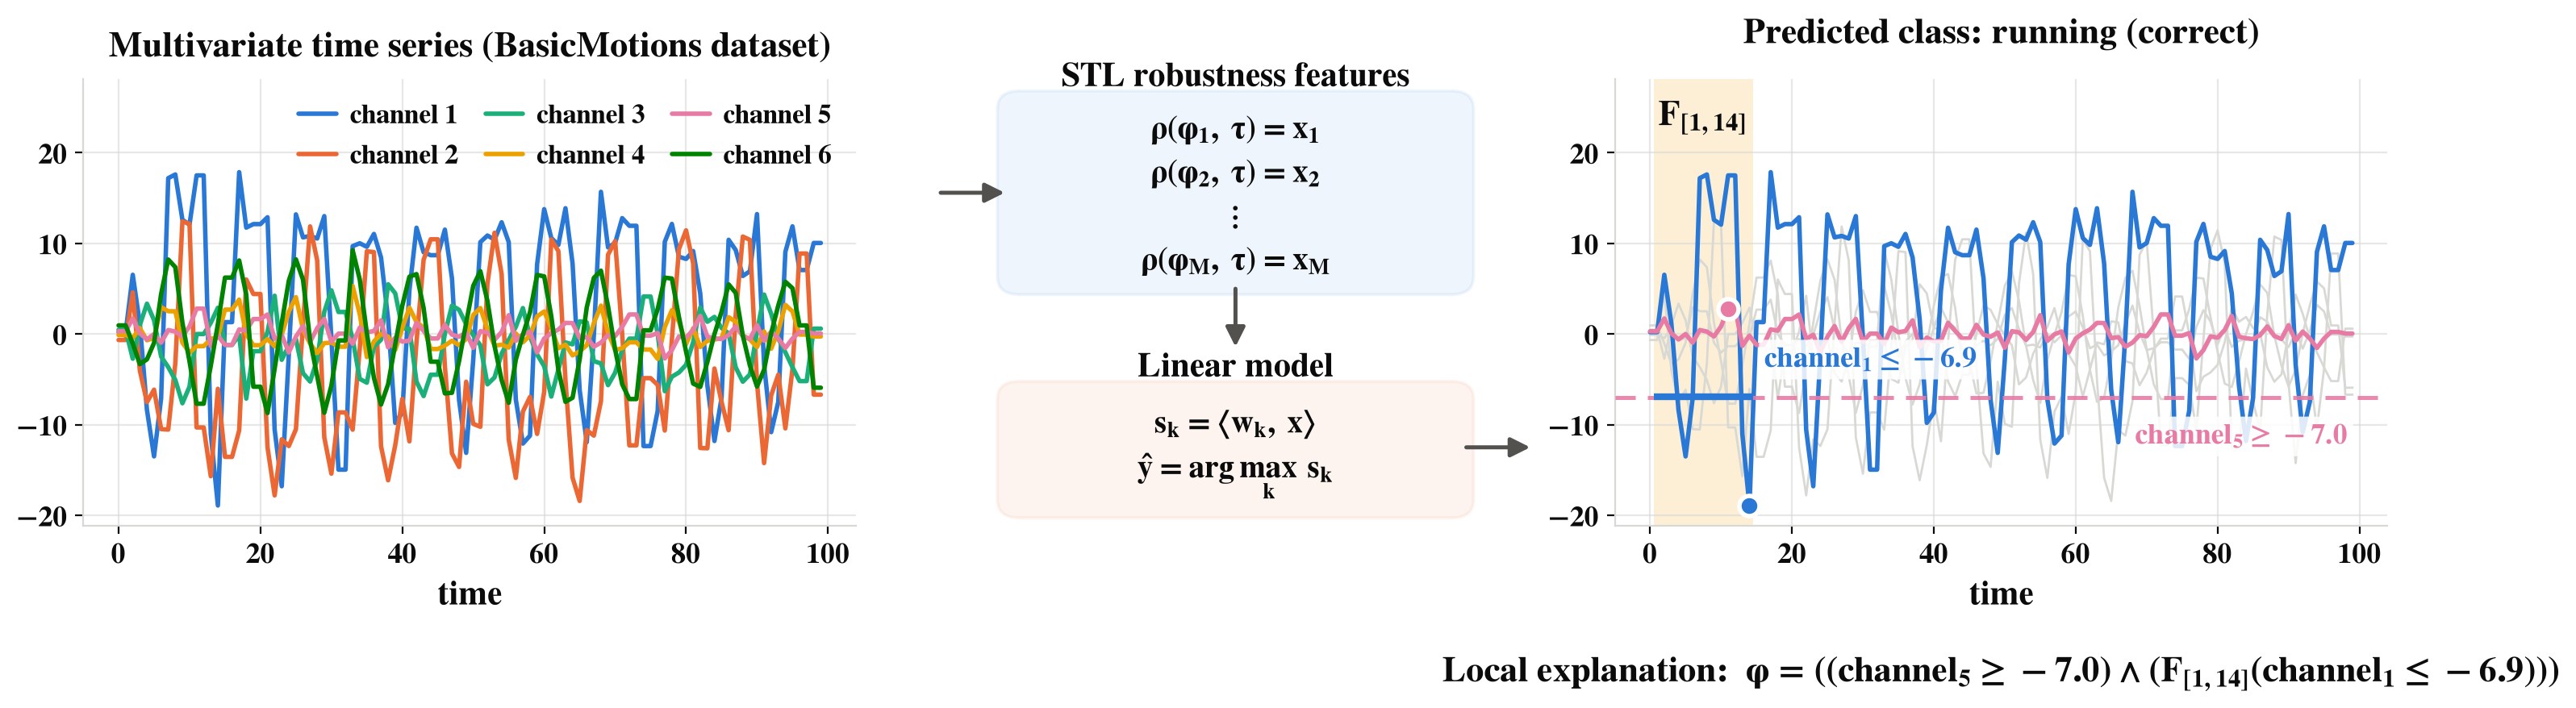
\includegraphics[width=\linewidth]{images/method_story.png}
\end{tikzfigure}
}

\begin{columns}

\column{0.5}
\block{Conclusion \& Future Work}{
  \begin{itemize}
    \item Every feature is an interpretable STL property.
    \item Explanations are STL formulae derived from model weights.
    \item Interpretability costs $2.1$ accuracy points against ROCKET, and buys
          local explanations of $85.8\%$ precision at depth ${\sim}3$.
    \item Next: simplification of global explanations, whose depth grows with
          the number of disjuncts (up to $12$ here).
    \item Next: differentiable tuning of thresholds instead of the median-based
          reparametrization.
  \end{itemize}
}

\column{0.5}
\block{References}{
  \small
  \begin{thebibliography}{9}
  \bibitem{rocket} Dempster, A., Petitjean, F., Webb, G.~I.
    \textit{ROCKET: exceptionally fast and accurate time series classification
    using random convolutional kernels}.
    Data Mining and Knowledge Discovery 34(5), 1454--1495, 2020.
  \bibitem{anchors} Ribeiro, M.~T., Singh, S., Guestrin, C.
    \textit{Anchors: High-Precision Model-Agnostic Explanations}.
    AAAI, 1527--1535, 2018.
  \bibitem{stl} Maler, O., Nickovic, D.
    \textit{Monitoring Temporal Properties of Continuous Signals}.
    FORMATS/FTRTFT, LNCS 3253, 152--166, 2004.
  \bibitem{glmnet} Friedman, J., Hastie, T., Tibshirani, R.
    \textit{Regularization Paths for Generalized Linear Models via Coordinate
    Descent}. Journal of Statistical Software 33(1), 1--22, 2010.
  \bibitem{uea} Bagnall, A., Dau, H.~A., Lines, J., Flynn, M., Large, J.,
    Bostrom, A., Southam, P., Keogh, E.
    \textit{The UEA multivariate time series classification archive, 2018}.
    arXiv:1811.00075, 2018.
  \end{thebibliography}
}
\end{columns}

\block{}{
  \centering\large Paper \& code: \texttt{https://your-link-here} \quad | \quad Acknowledgments: funding sources.
}

\end{document}
